\documentclass[times, utf8, zavrsni]{fer}
\usepackage{booktabs}

\begin{document}

% TODO: Navedite broj rada.
\thesisnumber{012}

% TODO: Navedite naslov rada.
\title{Višezadaćni rad, sinkronizacijski mehanizmi i upravljanje spremnikom u Android okruženju}

% TODO: Navedite vaše ime i prezime.
\author{Hrvoje Kozak}

\maketitle

% Ispis stranice s napomenom o umetanju izvornika rada. Uklonite naredbu \izvornik ako želite izbaciti tu stranicu.
% \izvornik

% Dodavanje zahvale ili prazne stranice. Ako ne želite dodati zahvalu, naredbu ostavite radi prazne stranice.
\zahvala{}

\tableofcontents

\chapter{Uvod}
Uvod rada. Nakon uvoda dolaze poglavlja u kojima se obrađuje tema.

\chapter{Upravljanje memorijom}
\section{Kako operacijski sustav Android upravlja memorijom}
\paragraph{}
Android ne nudi prostor za zamjenu \textit{(engl. swap)} za memoriju, već u tu svrhu koristi straničenje \textit{(engl. paginig)} i mapiranje memorije \textit{(engl. memory-mapping)}.\\

\textbf{Straničenje} \textit{(engl. paging)} je način na koji se spremaju i dohvaćaju podaci s vanjskog spremnika u glavnu memoriju. Operacijski sustav će te podatke dohvaćati u blokovima iste veličine i jedan takav blok zove se stranica. Ova tehnika isto tako važan je dio u implementaciji virtualne memorije, gdje se onda korištenjem vanjskog spremnika omogućava programima da prerastu dostupnu fizičku memoriju.\\

\textbf{Datoteka mapirane memorije} \textit{(engl. Memory-mapped file)} je segment virtualne memorije kojem se dodjeljuje direktna bajt po bajt korelacija s nekom datotekom ili sličnim resursom. Tipično je to datoteka koja se nalazi fizički na disku, ali može biti i uređaj ili objekt dijeljene memorije. Nakon povezanog mapiranja između datoteke i virtualne memorije aplikaciji se omogućava da tretira mapirani dio kao primarnu memoriju.\\

To bi značilo da kada god se koristi memorija, bilo alociranjem novih objekata ili korištenjem mapiranih stranica, ona ostaje unutar radne memorije i ne sprema se na vanjsku stranicu. Stoga, jedini način da se kompletno otpusti memorija iz aplikacije je otpuštanje referenci na objekte koji su trenutno u memoriji, nakon čega će ta memorija biti počišćena u procesu prikupljanja otpada. Postoji jedna iznimka, datoteke mapirane u sustav koje nisu mijenjane (npr. Izvorni kod) mogu se izvaditi u stranicu izvan radne memorije ako sustav trenutno želi koristiti tu memoriju u druge svrhe.

\subsection{Dijeljenje memorije}
\paragraph{}
Da bi uspjeli ubaciti sve u memoriju što nam je potrebno, procesi su primorani dijeliti stranice radnog spremnika. Samo dijeljenje stranica između procesa događa se na sljedeći način:

\begin{enumerate}
\item
Svaki proces aplikacije se račva \textit{(engl. fork)} od glavnog postojećeg procesa zvanog Zigota. Proces Zigote započinje svoj život odmah nakon što se uređaj pokrene \textit{(engl. boot)} i učita izvorni kod radnog okruženja \textit{(engl. framework)} i resurse. Prilikom pokretanja novog procesa aplikacije, sustav račva Zigotu, te učita i pokrene izvorni kod aplikacije u novom procesu. Time se dobiva efekt da većina RAM stranica alociranih za radno okruženje i resurse bude dijeljena na svim živim procesima.

\item
Većina statičnih podataka je mapirano u proces. Na taj su način ti podaci automatski podijeljeni s drugim procesima i mogu se zapisati u stranice ako je potrebno.

\item
Na puno mjesta, Android dijeli isti dinamički radni spremnik na više procesa pomoću eksplicitno alocirane regije djeljene memorije (korištenjem \textit{ashmem} ili \textit{gralloc} naredbi).
\end{enumerate}

\subsection{Alociranje i oslobađanje memorije aplikacije}
\paragraph{}
Za svaki proces, hrpa virtualne mašine Dalvik limitirana je na samo jednu virtualnu memoriju. To određuje logičku veličinu hrpe, koja raste po potrebi i koja ne mora nužno biti jednaka količini fizičke memorije koju hrpa koristi. Dalvik hrpa ne sažima logičku veličinu hrpe, što znači da ne radi nikakvu fragmentaciju. Jedino u slučaju pojavljivanja neiskorištenog prostora na kraju hrpe operacijski sustav može sažeti logičku veličinu hrpe.\\

Što se tiče fizičke memorije koju koristi hrpa, ona se može smanjiti. Nakon prikupljanja smeća, Dalvik prolazi kroz hrpu i nalazi nekorištene stranice koje onda vraća nazad \textit{kernelu} (naredbom \textit{madvise}). Treba primijetiti da ako imamo alokacije uparene s oslobađanjem, kod velikih komada memorije može se očekivati da će sva memorija biti vraćena. S druge strane manje efektivan je slučaj kada se promatraju manje alokacije jer stranica korištena za manje alokacije može biti dijeljena s nečime što se još nije oslobodilo.

\subsection{Ograničavanje memorije aplikacije}
\paragraph{}
Da bi održao funkcionalno više-dretveno (engl. multi-threading) okruženje, Android svakoj aplikaciji postavlja limit na njezinu veličinu hrpe. Taj limit varira i ovisi o samom uređaju, a baziran je na ukupnoj količini radne memorije na uređaju. U slučaju da aplikacija pokuša alocirati memoriju u trenutku kada je već dosegla svoj limit, dobiti će \textit{OutOfMemoryError}.\\

Provjera slobodnog prostora na hrpi može se pozvati \textit{getMemoryClass()} metoda. Ona će vratiti \textit{integer} koji pokazuje količinu slobodnih megabajta na hrpi za našu aplikaciju.

\subsection{Mijenjanje aplikacije od strane korisnika}
\paragraph{}
Kao što smo rekli Android nema prostor za zamjenu. Iz tog razloga, kada se korisnik prebacuje iz jedne aplikacije u drugu, Android sprema trenutno nevidljive procese u LRU \textit{(engl. Least Recently Used)} priručnu memoriju \textit{(engl. cache)}. Znači nakon što korisnik napusti aplikaciju, proces se ne ubija nego se sprema u priručnu memoriju sa svrhom ponovnog korištenja i bržih promjena aplikacija na uređaju.\\

Naravno dok se aplikacija ne koristi, pošto je spremljena u priručnoj memoriji, ona još uvijek koristi memorijski prostor. Ako sustavu nedostaje memorije, može odlučiti ubiti jednu od aplikacija u priručnoj memoriji. Odluku će donijeti na temelju procjene koja je aplikacija najmanje korištena u posljednje vrijeme, ili  koja od njih agresivno konzumira memoriju.

\pagebreak
\section{Upravljanje memorijom u Android aplikacijama}
\paragraph{}
Pri izradi Android aplikacija treba biti svijestan ograničenja memorije tokom svih faza razvoja, pa čak i prilikom izrade dizajna aplikacije neposredno prije samog početka razvoja. Takvim pristupom izbjegava se jako puno grešaka \textit{(engl. bug)} i curenja memorije \textit{(engl. memory leak)}, te se štedi vrijeme samog razvoja aplikacije. Postoje razne tehnike i dobre prakse vezane uz dizajn i pisanje koda koje povlače bolju kvalitetu same aplikacije i manje problema s memorijom, a u nastavku će se proći kroz one najbitnije.

\subsection{Pažljivo baratanje servisima}
\paragraph{}
Pri korištenju nekog servisa za odrađivanje posla u pozadini, mora se jako paziti da  ne ostane pokrenut u trenucima kada ne obavlja aktivno niti jedan posao. Isto tako ne smije se dogoditi da servis procuri, što se događa kada ga se zaboravi zaustaviti nakon obavljenog posla. Takav propust smatra se jednom od najgorih grešaka kod upravljanja memorijom jer ne samo da će aplikacija lošije funkcionirati, nego će i korisnici primijetiti neočekivana ponašanja i pobrisati aplikaciju s uređaja.\\

Najbolji način za limitiranje životnog spektra servisa je korištenje \textit{IntentService} klase, koja će se sama počistiti odmah nakon što odradi stvar zbog koje je pozvana.

\subsection{Otpuštanje memorije}
\paragraph{}
U bilo kojem trenutku života aplikacije, ugrađeni poziv \textit{(engl. callback)} \textit{onTrimMemory()} obavještava kada sveukupna memorija uređaja postaje premala. Na taj ugrađeni poziv trebalo bi odgovoriti otpuštanjem memorije resursa koji se drže u aplikaciji, a odluka o tome koje i koliko resursa otpustiti donosi se s obzirom na zaprimljeni nivo memorije od strane \textit{onTrimMemory()}. Nivoi memorije su sljedeći:

\paragraph{•}
\verb|TRIM_MEMORY_UI_HIDDEN|\\
Ovo je jedna od najvažnijih zastavica i indicira da je korisničko sučelje \textit{(engl. User Interface, UI)} trenutno skriveno od korisnika (npr. kada se korisnik navigira u drugu aplikaciju). To je signal da se trebaju osloboditi svi resursi koje trenutno koristi UI i tako znatno povećati kapacitet operacijskog sustava za spremanje procesa u priručnu memoriju, što je u krajnjoj liniji direktno poboljšanje kvalitete korisničkog korištenja aplikacije \textit{(engl. User Experience, UX)}.

\paragraph{•}
\verb|TRIM_MEMORY_RUNNING_MODERATE|\\
Naša aplikacija nije direktno ugrožena, sustav javlja da je slab s memorijom i počinje aktivno ubijati procese u LRU priručnoj memoriji.

\paragraph{•}
\verb|TRIM_MEMORY_RUNNING_LOW|\\
Naša aplikacija nije direktno ugrožena, sustav javlja da je puno slabiji s memorijom i ovdje bi se trebali već poćeti oslobađati nekorišteni resursi u aplikaciji.

\paragraph{•}
\verb|TRIM_MEMORY_RUNNING_CRITICAL|\\
Naša aplikacija još uvijek živi, ali sustav je već ubio većinu procesa u LRU priručnoj memoriji. Ovdje se trebaju otpustiti svi resursi koji nisu krucijalni za nastavak rada aplikacije.\\

\noindent
Ukoliko je naš proces već u priručnoj memoriji možemo očekivati sljedeće zastavice:

\paragraph{•}
\verb|TRIM_MEMORY_BACKGROUND|\\
Sustav je slab s memorijom, a naš proces je negdje na početku LRU liste. Iako naš proces nema prevelik rizik da bude uništen ubrzo, ovo je signal da se LRU priručna memorija već počinje čistiti i ovdje bi trebali osloboditi sve resurse koje je kasnije lako povratiti.

\paragraph{•}
\verb|TRIM_MEMORY_MODERATE|\\
Sustav je slab s memorijom, a naš proces je negdje na sredini LRU liste i postoji dobra šansa da se naš proces uništi ako proces zatraži još dodatne memorije.

\paragraph{•}
\verb|TRIM_MEMORY_COMPLETE|\\
Sustav je slab s memorijom, a naš proces je prvi koji će biti uništen ako sustav u tom trenutku ne uspije osloboditi dovoljno memorije. Ovdje treba otpustiti apsolutno sve što nije krucijalno za nastavak rada aplikacije.\\

Ovaj \textit{onTrimMemory()} ugrađeni poziv je dodan tek u API verzije 14 tako da za starije verzije uređaja treba koristiti \textit{onLowMemory()} ugrađeni poziv koji se u principu ponaša isto kao i \verb|TRIM_MEMORY_COMPLETE| \textit{event}.

\subsection{Provjera dostupne memorije}
\paragraph{}
Kako je svaki android uređaj drukčiji i njegova količina radne memorije varira, isto tako mijenja se i limit veličine hrpe za svaku aplikaciju na uređaju. U slučaju da aplikacija pokuša alocirati memoriju u trenutku kada je već dosegla svoj limit, dobiti će \textit{OutOfMemoryError}, a pozivom na \textit{getMemoryClass()} dobit će se procjena dostupne memorije za aplikaciju u megabajtima.\\

U posebnim slučajevima može se zatražiti veća količina hrpe postavljanjem atributa \textit{largeHeap} na \textit{true} unutar \textit{manifest} \verb|<application>| taga. Tada se procjena dostupne memorije za tu veću hrpu dobiva pozivom \textit{getLargeMemoryClass()} metode.\\

Naravno to se nikako ne smije koristiti kao lako rješenje svaki puta kada se ostane bez memorije. Ovakav pristup namijenjen je malom broju aplikacija koje mogu opravdati potražnju za većom količinom memorije.

\subsection{Skaliranje bitmapa}
\paragraph{}
Prilikom učitavanja \textit{bitmap} datoteke, cilj je u memoriji držati samo rezoluciju koja nam treba za ekran trenutnog uređaja. Ako je originalna \textit{bitmap} datoteka prevelika, skalirat ćemo ju na željenu veličinu. Ovime se štedi jako puno memorije jer količina memorije za držanje \textit{bitmap} datoteke raste kvadratno s porastom veličine grafike (jer rastu X i Y osi).

\subsection{Optimizirani spremnici podataka}
\paragraph{}
Radno okruženje Android nam nudi strukture za spremanje podataka koje su optimizirane za Android OS, kao na primjer \textit{SparseArray, SparseBooleanArray i LongSparseArray}. Ako uzmemo za primjer implementaciju \textit{HashMap} strukture, ona može biti jako neugodna za memoriju jer prilikom svakog mapiranja stvara novi objekt. S druge strane \textit{SparseArray} klase su optimizirane tako da izbjegavaju potrebu automatske konverzije iz primitiva u klasu objekta \textit{(engl. autoboxing)}(npr. int u Integer) ključa, a ponekad i same vrijednosti.\\

Isto tako možemo iskoristiti i bazične \textit{Java} nizove kada to ima smisla.

\subsection{Dodatni troškovi memorije}
\paragraph{}
U izradi aplikacije jedna od najbitnijih stvari koje trebamo pripaziti je cijene i dodatni troškovi \textit{(engl. overhead)} jezika i radnog okruženja koje koristimo. Često se ljudi naviknu uzimati stvari zdravo za gotovo i rade greške koje na prvi pogled izgledaju nevino, dok ustvari troše veliku količinu memorije.

\paragraph{•}
Enumeracije \textit{(engl. Enumerations, Enum)} često zahtjevaju i do duplo više memorije od statičkih konstanta. Njih bi svakako trebali izbjegavati.

\paragraph{•}
Svaka klasa u \textit{Javi} koristi približno 500 bajta koda.

\paragraph{•}
Svaka instanca klase ima 12-16 bajta dodatnog troška u radnom spremniku.

\paragraph{•}
Stavljanje jednog unosa u \textit{HashMap}, zahtjeva alokaciju još jednog dodatnog objekta veličine 32 bajta.\\

Iako u prvu ruku ne izgleda kao prevelika štednja, kada se ovakve sitnice  skaliraju to jako brzo postaje veliki problem iz perspektive memorije.

\subsection{Apstrakcija koda}
\paragraph{}
Iako je apstrakcija koda dobra praksa u programiranju jer svojom fleksibilnošću olakšava održavanje aplikacije, ona dolazi s cijenom, a cijena je puno veća količina koda koji se treba izvesti, što povlači za sobom više radne memorije. Ako apstrakcije ne olakšavaju strukturu i fleksibilnost koda moraju se izbjegavati, jer će memorija biti jako zahvalna na tome.

\subsection{Mehanizam za serijalizaciju Protobuffs}
\paragraph{}
\textit{Protobuffs (Protocol buffers)} je mehanizam razvijen od strane \textit{Google-a} za serijalizaciju struktura podataka neovisni o jeziku i platformi. Nešto poput XML-a, međutim puno brži, manji i jednostavniji. Ako se koristi u kodu, na Android operacijskom sustavu uvijek bi se trebala uzeti nano verzija protobuffs mehanizma na klijentskoj strani koda. Time se značajno smanjuje korištenje memorije i veličina APK arhive, te se pritom ubrzava samo izvođenje programa.

\subsection{Ubrizgavanje zavisnosti}
\paragraph{}
Kada se koristi neko radno okruženje za ubrizgavanje zavisnosti (engl. dependency injection) kao \textit{Dagger} ili \textit{Guice}, iako olakšavaju samo kodiranje i testiranje aplikacije kontrolom dependency-a, moramo paziti na činjenicu da oni rade jako puno inicijalizacije procesa tijekom skeniranja našeg koda tražeći anotacije i time mapiraju u radnu memoriju značajnu količinu koda iako nam taj kod u memoriji i ne treba. Te stranice su mapirane u čistu memoriju kako bi ih Android mogao počistiti, no to će se dogoditi tek nakon što stranice odstoje u memoriji neko vrijeme nekorištene.

\subsection{Eksterne biblioteke}
\paragraph{}
Na eksterne biblioteke treba uvijek posebno paziti, pogotovo kada ih se koristi više u jednom projektu. Prvo se dolazi do problema kada biblioteka nije optimizirana za korištenje na mobilnim uređajima, u kojem će se slučaju morati preuzeti pisanje optimizacije i održavanje tog koda. S druge strane i onda kada su biblioteke navodno optimizirane za mobilne uređaje, tu imamo potencijalni problem kada više njih rade istu stvar na različite načine i javljaju se veliki dodatni troškovi memorije. Na primjer, ako koristimo dvije biblioteke s različitim implementacijama za \textit{logging, caching, analytics} i slično.

\subsection{Proguard}
\paragraph{}
Proguard je jako koristan alat koji smanjuje, optimizira i pomućuje (engl. obfuscates) kod. To radi tako da makne kod koji se ne koristi, te zamijeni imena varijabli, klasa i metoda sa semantički besmislenim imenima. 

\subsection{Poravnavanje finalne APK arhive}
\paragraph{}
Nakon što se potpiše produkcijska verzija aplikacije mora se i poravnati \textit{zipalign} alatom. U protivnom, aplikacija će trošiti znatno više radne memorije, jer se resursi neće moći automatski mapirati iz APK-a.

\begin{center}
\verb|zipalign [-f] <alignment> infile.apk outfile.apk|
\end{center}

Za \textit{alignment} parametar koristi se 4 bajta na android okruženju, a zastavica –f forsira prepisivanje rezultata preko postojeće \textit{outfile.apk} datoteke.

\subsection{Analiza korištenja radne memorije}
\paragraph{}
Da bi se dobio bolji uvid u funkcionalnost naše aplikacije, svaki stabilan build bilo bi dobro analizirati.
Prvi I najjednostavniji način je čitanje informacijskih poruka (engl. log) sakupljača smeća. Dok Dalvik svaki put printa poruke sakupljača smeća, ART printa samo one koje su eksplicitno zahtjevane.\\

Druga stvar koja nam pomaže je Android Debug Monitor u Android Studiu koji prikazuje raznovrsne informacije o stanju memorije i uređaja općenito.\\

\begin{figure}[ht!]
\centering
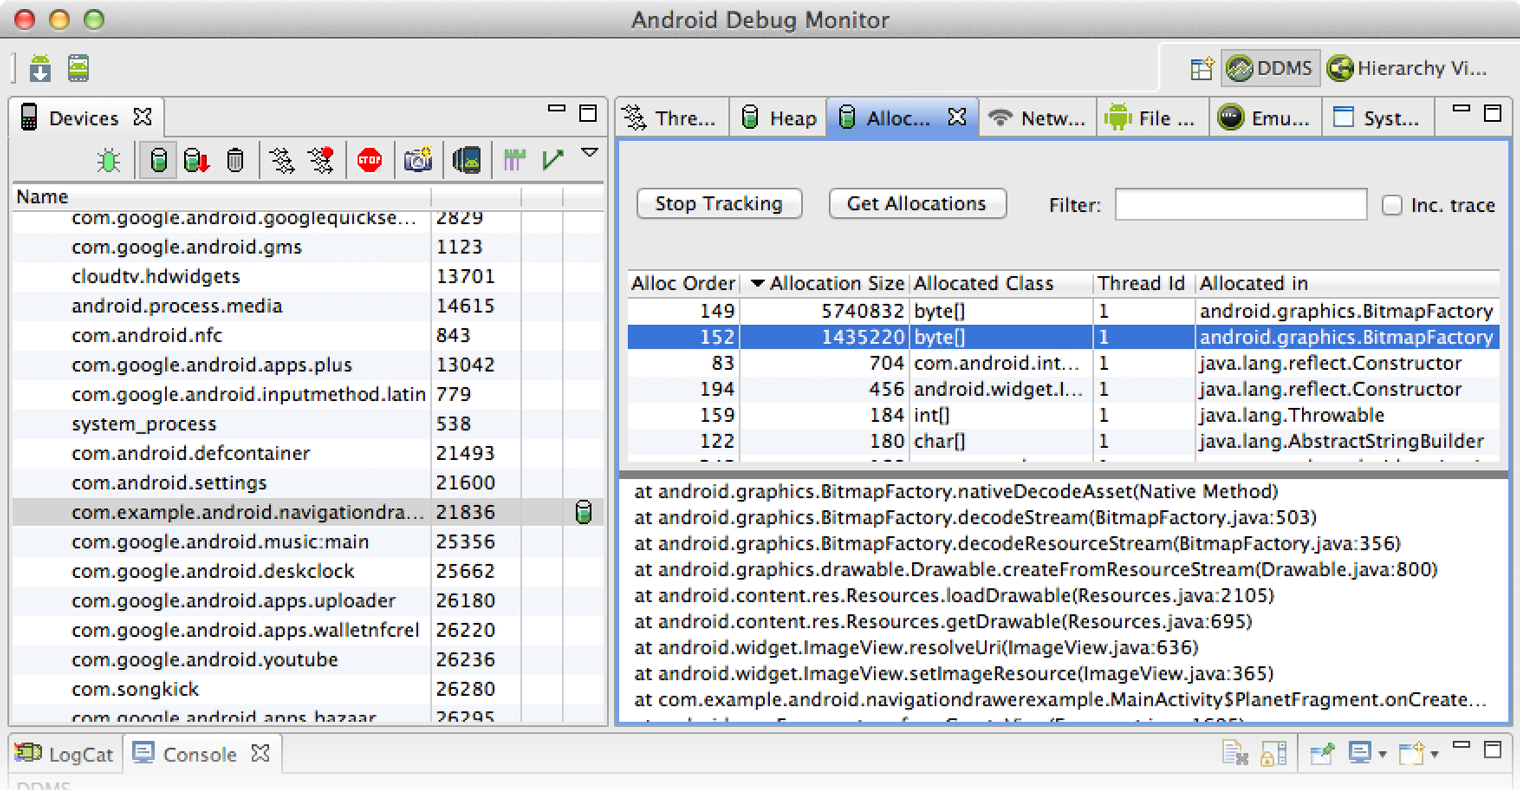
\includegraphics[width=140mm]{img/android-debug-monitor.png}
\caption{Android debug monitor.}
\label{overflow}
\end{figure}

Za detaljniju analizu može se pogledati kako je memorija naše aplikacije podijeljena po raznim tipovima alokacije radnog spremnika pomoću \textit{adb} naredbe:

\begin{center}
\verb=adb shell dumpsys meminfo <package_name | pid> [-d]=
\end{center}
koja će dati rezultat sličan ovome:

\begin{figure}[ht!]
\centering
\begingroup
    \fontsize{9pt}{12pt}\selectfont
		\begin{verbatim}
		** MEMINFO in pid 18227 [com.google.android.apps.maps] **
		                   Pss  Private  Private  Swapped     Heap     Heap     Heap
		                 Total    Dirty    Clean    Dirty     Size    Alloc     Free
		                ------   ------   ------   ------   ------   ------   ------
		  Native Heap    10468    10408        0        0    20480    14462     6017
		  Dalvik Heap    34340    33816        0        0    62436    53883     8553
		  ...
		  ...
		        TOTAL   216524   208232     4384        0    82916    68345    14570
\end{verbatim}
\endgroup
%\includegraphics[width=120mm]{img/example.png}
\caption{Analiza memorije procesa.}
\label{overflow}
\end{figure}

\noindent
i ovdje nam je bitno raspoznati dvije stvari:


\paragraph{•}
Privatni čisti i prljavi radni spremnik \textit{(engl. Private Clean and Dirty RAM)}\\
Ovo je količina memorije koju koristi naš proces i to je onaj dio memorije koji sustav može dobiti nazad nakon uništavanja istog. Ovdje je najbitnije gledati prljavi dio radnog spremnika, koji je ujedno i najskuplji, jer se tim djelom koristi samo naš process i ne može se straničiti na disk.

\paragraph{•}
Proporcionalna veličina skupa \textit{(engl. Proportional Set Size, PSS)}\\
Ovo je količina memorije koju koristi naša aplikacija uzimajući u obzir dijeljenje stranica kroz više procesa. Svaka stranica koja je jedinstvena za naš process direktno pridonosi ovoj vrijednosti, dok ostale stranice koje se dijele s drugim procesima doprinose proporcionalnu vrijednost dijela kojeg zauzimaju.

\subsection{Korištenje više procesa}
\paragraph{}
Iako velika većina aplikacija ne bi smjela koristiti više procesa u isto vrijeme, jer bi se mogli opeći i umjesto smanjenja, povećati iznos otiska \textit{(engl. footprint)} aplikacije u radnoj memoriji. No ako se ipak ide ovim putem mora se obratiti pažnja kakve će to utjecaje imati na našu memoriju.\\

Za ilustraciju posljedica zamislit će se jedan prazni process koji ne radi apsolutno ništa, i takav process ima dodatnih 1.4MB otiska u radnoj memoriji.

\begin{figure}[ht!]
\centering
\begingroup
    \fontsize{8pt}{12pt}\selectfont
		\begin{verbatim}
adb shell dumpsys meminfo com.example.android.apis:empty

** MEMINFO in pid 10172 [com.example.android.apis:empty] **
                Pss     Pss  Shared Private  Shared Private    Heap    Heap    Heap
              Total   Clean   Dirty   Dirty   Clean   Clean    Size   Alloc    Free
             ------  ------  ------  ------  ------  ------  ------  ------  ------
  Native Heap     0       0       0       0       0       0    1864    1800      63
  Dalvik Heap   764       0    5228     316       0       0    5584    5499      85
 Dalvik Other   619       0    3784     448       0       0
        Stack    28       0       8      28       0       0
    Other dev     4       0      12       0       0       4
     .so mmap   287       0    2840     212     972       0
    .apk mmap    54       0       0       0     136       0
    .dex mmap   250     148       0       0    3704     148
   Other mmap     8       0       8       8      20       0
      Unknown   403       0     600     380       0       0
        TOTAL  2417     148   12480    1392    4832     152    7448    7299     148
		\end{verbatim}
\endgroup
%\includegraphics[width=120mm]{img/example.png}
\caption{Analiza memorije praznog procesa.}
\label{overflow}
\end{figure}

Može se primijetiti da veličina nije baš zanemariva, i isto tako brzo i raste porastom kompleksnosti posla tog procesa. Na primjer, process koji prikazuje jedan \textit{Activity} sa tekstom će zauzeti 4MB, što je tri puta više, i to samo za prikazivanje običnog teksta na UI.\\

Ovime dolazimo do konkretnog zaključka, ako već moramo podijeliti aplikaciju u procese, isključovo jedan process mora biti zadužen za UI, a ostali moraju izbjegavati bilo kakvo korištenje UI elemenata, jer u suprotnom ćemo napuniti memoriju u kratkom roku.\\

Dodatno pošto se aplikacija vrti u više procesa mora se puno više fokusa uložiti u optimizaciju korištenja memorije u kodu jer se u ovom slučaju svaki propust replicira na druge procese i stvara sve veći problem.


\chapter{Zaključak}
Zaključak.

\bibliography{literatura}
\bibliographystyle{fer}

\begin{sazetak}
Sažetak na hrvatskom jeziku.

\kljucnerijeci{Ključne riječi, odvojene zarezima.}
\end{sazetak}

% TODO: Navedite naslov na engleskom jeziku.
\engtitle{Title}
\begin{abstract}
Abstract.

\keywords{Keywords.}
\end{abstract}

\end{document}
